

\documentclass{article}

\usepackage[margin=1in]{geometry} % Please keep the margins at 1.5 so that there is space for grader comments.
\usepackage{amsmath,amsthm,amssymb,hyperref, mathdots, graphicx, listings}

\newcommand{\R}{\mathbb{R}}  
\newcommand{\Z}{\mathbb{Z}}
\newcommand{\N}{\mathbb{N}}
\newcommand{\Q}{\mathbb{Q}}

\newenvironment{theorem}[2][Theorem]{\begin{trivlist}
\item[\hskip \labelsep {\bfseries #1}\hskip \labelsep {\bfseries #2.}]}{\end{trivlist}}
\newenvironment{lemma}[2][Lemma]{\begin{trivlist}
\item[\hskip \labelsep {\bfseries #1}\hskip \labelsep {\bfseries #2.}]}{\end{trivlist}}
\newenvironment{claim}[2][Claim]{\begin{trivlist}
\item[\hskip \labelsep {\bfseries #1}\hskip \labelsep {\bfseries #2.}]}{\end{trivlist}}
\newenvironment{problem}[2][Problem]{\begin{trivlist}
\item[\hskip \labelsep {\bfseries #1}\hskip \labelsep {\bfseries #2.}]}{\end{trivlist}}
\newenvironment{proposition}[2][Proposition]{\begin{trivlist}
\item[\hskip \labelsep {\bfseries #1}\hskip \labelsep {\bfseries #2.}]}{\end{trivlist}}
\newenvironment{corollary}[2][Corollary]{\begin{trivlist}
\item[\hskip \labelsep {\bfseries #1}\hskip \labelsep {\bfseries #2.}]}{\end{trivlist}}

\newenvironment{solution}{\begin{proof}[Solution]}{\end{proof}}

\begin{document}

\large % please keep the text at this size for ease of reading.

% ------------------------------------------ %
%                 START HERE             %
% ------------------------------------------ %

{\Large% Replace with appropriate page number 
\hfill Max Sours}

\begin{center}
{\Large PHY407 Final Project: N-body Problems} % Replace "Author's Name" with your name
\end{center}
\vspace{0.05in}

{\Large \textbf{Computational Background}}

\textbf{Euler Methods}

For a system of 1st order ODEs:

$$\frac{d\mathbf{v}}{dt} = \mathbf{F}(\mathbf{x}), \frac{d\mathbf{x}}{dt} = \mathbf{v}$$

Forward Euler uses the following formula to integrate the system.

$$\mathbf{v_{i+1}} = \mathbf{v_i} + \mathbf{F}(\mathbf{x_i})\Delta t$$
$$\mathbf{x_{i+1}} = \mathbf{x_i} + \mathbf{v_i}\Delta t$$

for some timestep $\Delta t$. Forward Euler is often unstable, but there is a slightly different version that is much more stable.

Semi-Implicit Euler integrates the system like so:

$$\mathbf{v_{i+1}} = \mathbf{v_i} + \mathbf{F}(\mathbf{x_i})\Delta t$$
$$\mathbf{x_{i+1}} = \mathbf{x_i} + \mathbf{v_{i+1}}\Delta t$$

The difference being that in the last equation, $\mathbf{v_{i+1}}$ is used instead of $\mathbf{v_i}$.

\textbf{Verlet Method}

Another method of solving the system

$$\frac{d\mathbf{v}}{dt} = \mathbf{F}(\mathbf{x}), \frac{d\mathbf{x}}{dt} = \mathbf{v}$$

Is the following:

$$\mathbf{x_{i + 1}} = \mathbf{x_i} + \mathbf{v_i} \Delta t + \frac{1}{2}\mathbf{F}(\mathbf{x_i}) \Delta t^2$$
$$\mathbf{v_{i + 1}} = \mathbf{v_i} + \frac{1}{2}(\mathbf{F}(\mathbf{x_i}) + \mathbf{F}(\mathbf{x_{i+1}}))\Delta t$$

\textbf{Adaptive Runge-Kutta-Fehlberg}

The adaptive Runge-Kutta-Fehlberg algorithm uses a 4th order Runge-Kutta method along with a 5th order Runge-Kutta method to estimate the error. If the error exceeds the tolerance, decrease the timestep. Otherwise, increase the timestep.

{\Large \textbf{Physics Background}}

{\Large \textbf{Questions}}

\begin{enumerate}
	\item \textbf{Errors in n-Body Integration}
	
	\begin{enumerate}
		\item We will test the accuracy of several integration methods using a two-body system of the Sun and a large asteroid. Set the initial position of the asteroid to be 1 AU from the Sun and the initial velocity at 10 km/s. Remember that the center of mass and net momentum should both be 0.
		
		Nothing to submit.
		
		\item In Lab 1 you learned that the Semi-Implicit Euler (also called Euler-Cromer) method gave satisfactory results for the Sun-Mercury system (with the Sun being a fixed point). We will use this method to simulate the Sun-Asteroid system. Use the initial conditions from above and integrate the system over 300 days with a timestep of 1 hour (3600 s). Output plots of the positions of the Sun and the asteroid, and the total energy of the system over time. What does the energy plot tell you about the error in the system? Is Semi-Implicit Euler a good integration method?
		
		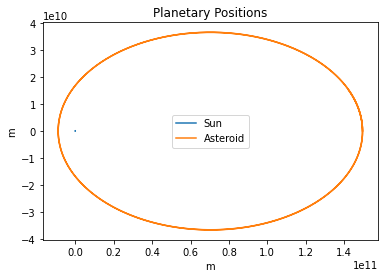
\includegraphics[scale = 0.8]{q1b_1.png}
		
		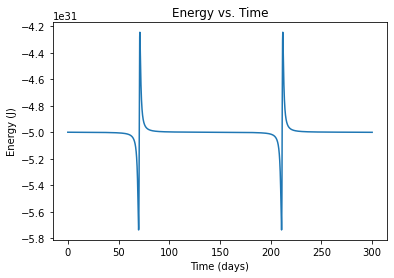
\includegraphics[scale = 0.8]{q1b_2.png}
		
		\item Repeat part (b) for the Verlet method. Report energy over time. You should generate a plot of positions to verify the algorithm is generating good results, but you don't need to report it. Is energy conserved at all times? When is energy not conserved?
		
		\item Implement the adaptive Runge-Kutta-Fehlberg method. Run the same simulation with a starting timestep of 2048 s (or any power of 2), an xtol of 100 km, and a vtol of 0.1 m/s. Output the energy plot and comment on the results. Additionally, plot time as a function of iterations. When is the algorithm taking smaller timesteps?
	\end{enumerate}

	\item \textbf{Integrating the Sun-Earth-Moon System}
	
	\begin{enumerate}
		\item Set up the initial conditions for the Sun-Earth-Moon system. We want the center of mass to be at the origin and for the total momentum of the system to be the zero vector. While we will assume all orbits occupy the same plane, your simulation will be in three dimensions. For the initial positions, make sure the Earth is 1 AU away from the sun and the Moon is 0.00257 AU away from the Earth. For the initial velocities, give the Earth the velocity needed for a circular orbit around the Sun, and give the Moon the velocity required for a circular orbit around the Earth. Remember that the total momentum of the system should be 0.
	\end{enumerate}
\end{enumerate}
% --1--d_1-----------------------------------------------
% Anything after the \end{document} will be ignored by the typesetting.
% ----------------------------------------------------

\end{document}

